% !TeX encoding = utf8
\documentclass[german,aspectratio=169]{beamer}
\usepackage{beamerthemeHM} 
\usepackage{graphicx}

% These are some nice colors that fit well together
\definecolor{midnightblue}{RGB}{10,10,44}
\definecolor{navyblue}{RGB}{0,0,120}
\definecolor{crimson}{RGB}{220,20,60}
\definecolor{mydarkgray}{RGB}{33,33,33}
\definecolor{myalgColor}{RGB}{99,99,99}
\definecolor{mygreen}{RGB}{85,168,104}
\definecolor{myorange}{RGB}{221,132,82}
\definecolor{myblue2}{rgb}{0.12156862745098039, 0.4666666666666667, 0.7058823529411765}
\definecolor{myblue3}{rgb}{0.2980392156862745, 0.4470588235294118, 0.6901960784313725}
\definecolor{myblue4}{rgb}{0.2823529411764706, 0.47058823529411764, 0.8156862745098039}
\definecolor{mybluebright}{rgb}{0.00784313725490196, 0.24313725490196078, 1.0}
\definecolor{myred}{RGB}{196,78,82}
\definecolor{mydarkgray}{RGB}{90,90,90}
\definecolor{mygray}{RGB}{179,179,179}
\definecolor{myviolet}{RGB}{129,114,178}
\definecolor{myblue}{RGB}{76,114,202}
\xdefinecolor{mybg}{rgb}{0.7419607843137255, 0.9027297193387159, 0.868958093041138}
\xdefinecolor{myRed}{rgb}{0.7686274509803922, 0.3058823529411765, 0.3215686274509804}
\xdefinecolor{prevColor}{rgb}{0.39215686274509803, 0.7098039215686275, 0.803921568627451}
\xdefinecolor{mylightblue}{rgb}{0.8584083044982699, 0.9134486735870818, 0.9645674740484429}

\definecolor{mybrightblue}{rgb}{0.00784313725490196, 0.24313725490196078, 1.0}
\definecolor{mybrightred}{rgb}{0.9098039215686274, 0.0, 0.043137254901960784}

\xdefinecolor{myalgColor}{rgb}{0.7686274509803922, 0.3058823529411765, 0.3215686274509804}

% hm colors
\xdefinecolor{hmred}{RGB}{252, 85, 85}

%
\xdefinecolor{colordefinition}{RGB}{0, 123, 255}
\xdefinecolor{colorexample}{RGB}{200, 200, 200}

% listing colors
\definecolor{codegreen}{rgb}{0,0.6,0}
\definecolor{codegray}{rgb}{0.5,0.5,0.5}
\definecolor{codepurple}{rgb}{0.58,0,0.82}
\definecolor{backcolour}{rgb}{0.95,0.95,0.92}

\definecolor{halfgray}{gray}{0.55}
\definecolor{ipython_frame}{RGB}{207, 207, 207}
\definecolor{ipython_bg}{RGB}{247, 247, 247}
\definecolor{ipython_red}{RGB}{186, 33, 33}
\definecolor{ipython_green}{RGB}{0, 128, 0}
\definecolor{ipython_cyan}{RGB}{64, 128, 128}
\definecolor{ipython_purple}{RGB}{170, 34, 255}

%packages%
\usepackage{savesym}
\usepackage{longtable}
\usepackage{listings}
\usepackage{placeins}
\usepackage{media9}
\usepackage{appendixnumberbeamer}
%\usepackage{multimedia}
%\usepackage{animate}
\usepackage[font=itshape,noorphans=true]{quoting}

%font
\usepackage{amsmath,amsfonts,amsthm,amssymb,mathtools,stmaryrd,xpatch}
\usepackage[T1]{fontenc}
\usepackage{marvosym} 
\usepackage{libertine}
\usepackage[libertine]{newtxmath}

% german symbols
\usepackage[utf8]{inputenc}

\usepackage{array}
\usepackage{makecell}
\usepackage{graphicx}
\usepackage{color}
\usepackage{emptypage}
\usepackage[toc,page]{appendix}
\usepackage{listings}

%\usepackage[format=plain, skip=5pt, labelfont=bf]{caption}
\usepackage{subfigure}
%\usepackage[labelfont=normalfont]{subcaption}
%\usepackage[ngerman,english]{babel}
\usepackage[ngerman]{babel}
%\usepackage{polyglossia}%german beamer commands
\usepackage{tikz}
\usetikzlibrary{%
	positioning,calc,trees,positioning,automata,arrows,chains,shapes.geometric,%
	decorations.pathreplacing,decorations.pathmorphing,shapes,%
	matrix,shapes.symbols%
}%
\let\openbox\undefined
\usepackage[vlined,linesnumbered,resetcount]{algorithm2e}
\usepackage[numbers]{natbib}
\usepackage{bussproofs}
\usepackage{stackengine}
\usepackage{enumitem}
\usepackage{framed}
\usepackage{url}
\urlstyle{same}
\usepackage[capitalise]{cleveref}
\usepackage{hyperref}

% Zahlen, Mengen, Intervalle, Addieren, Multiplizieren, Subtrahieren, Dividieren
\title{\huge Computational Thinking}
\subtitle{Algorithmisches Denken mithilfe des Jupyter-Ökosystems}
\author{\href{mailto:zoennchen.benedikt@hm.edu}{Dr. Benedikt Zönnchen} \\ \href{mailto:martin.hobelsberger@hm.edu}{Prof. Dr. Martin Hobelsberger}}
\date{19. Mai 2022}
\institute{
\includegraphics[height=15pt]{./figs/Hochschule_Muenchen_Logo}}
\begin{document}

\begin{frame}
 \titlepage
\end{frame}

\begin{frame}
	\frametitle{Überblick}
	\textbf{
	\begin{enumerate}[label = \arabic*.]
		\item Herausforderung
		\item Kurskonzeption
		\item Realisierung
		\begin{enumerate}[label = 3.\arabic*]
			\item Intuitiver Zugang
			\item Minimale technische Hürden
			\item Kontinuierliches Feedback
		\end{enumerate}
	\item Retrospektive
	\end{enumerate}
	}
\end{frame}

\begin{frame}
	\frametitle{Herausforderung}
	Vielfältige interdisziplinäre CSPlus / PlusCS Studiengänge der Hochschule München:
	\begin{enumerate}[label=$\bullet$]
		\item Digital Engineering
		\item Informatik und Design
		\item Geodata Science
		\item Data Science \& Scientific Computing
		\item $\ldots$ (in der Zukunft)
	\end{enumerate}
	$\Rightarrow$ Erhöhte Heterogenität der Studierenden
\end{frame}

\begin{frame}
	\frametitle{Herausforderung}
	Studierenden jener Studiengänge soll es möglich sein
	\begin{quoting}
		\glqq\textbf{Problemstellungen} zu \textbf{identifizieren}, \textbf{abstrakt} zu \textbf{modellieren}, sie dabei in \textbf{Teilprobleme} zu \textbf{zerlegen}, \textbf{Lösungsstrategien} zu \textbf{entwerfen} und auszuarbeiten und diese \textbf{formalisiert} \textbf{darzustellen}, sodass sie von einem Menschen (oder auch einem Computer) verstanden und ausgeführt werden können.\grqq
	\end{quoting}
	Kurz gesagt: Studierende sollen \textbf{Computational Thinking (CT)} beherrschen.
\end{frame}

\section{Kurskonzeption}

\begin{frame}
	\frametitle{Überblick}
		\begin{enumerate}[label = \arabic*.]
			\item Herausforderung
			\item \textbf{Kurskonzeption}
			\item Realisierung
			\begin{enumerate}[label = 3.\arabic*]
				\item Intuitiver Zugang
				\item Minimale technische Hürden
				\item Kontinuierliches Feedback
			\end{enumerate}
			\item Retrospektive
		\end{enumerate}
\end{frame}

\begin{frame}
	\frametitle{Was verstehen wir unter CT?}
	\begin{center}
		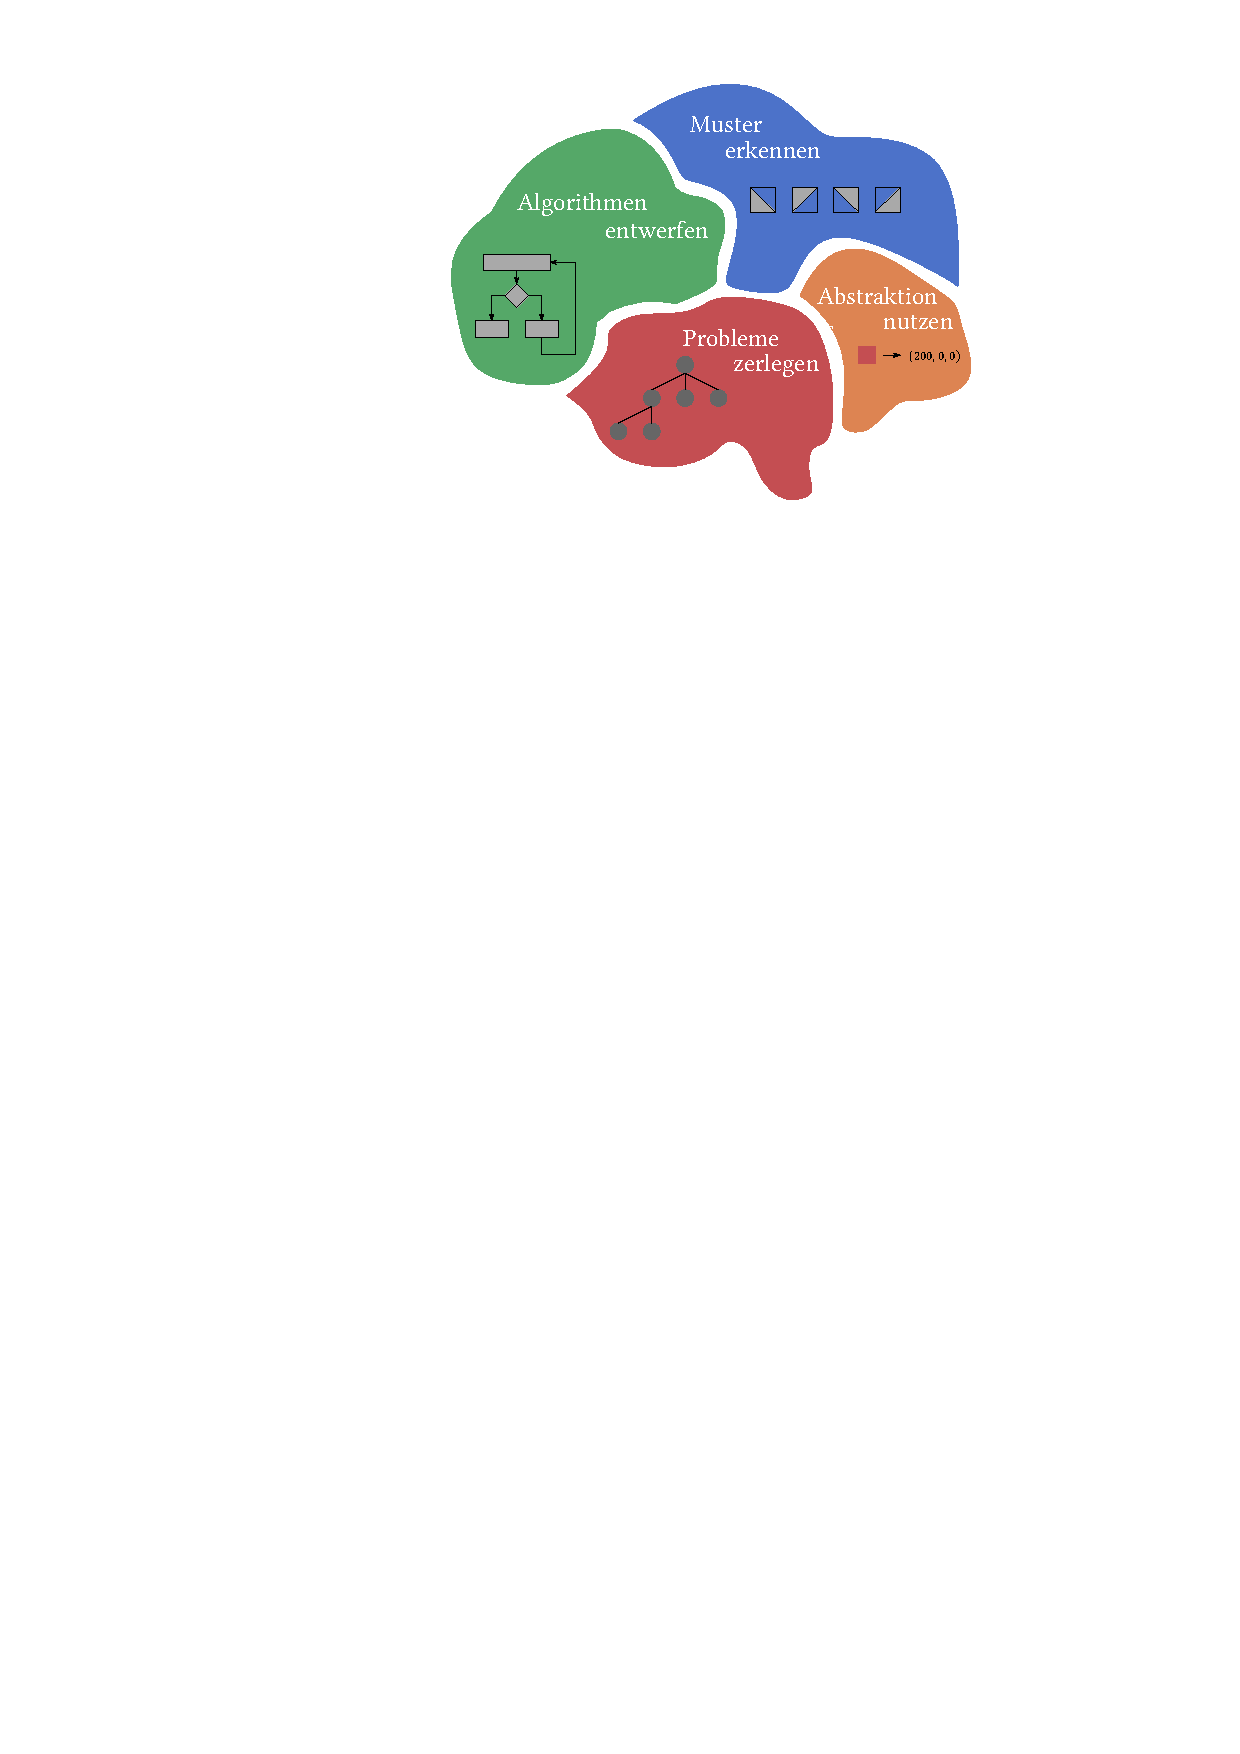
\includegraphics[width=0.6\textwidth]{./figs/ct-logo}
	\end{center}
\end{frame}

%\begin{frame}
%	\frametitle{Was verstehen wir unter CT?}
%	Computational Thinking
%	\begin{enumerate}[label=$\bullet$]
%		\item ist eine Aktivität,
%		\item bedeutet primär konzipieren (Programmierung als Mittel),
%		\item ist eine fundamentale Fähigkeit,
%		\item ist eine Denkweise des Menschen (nicht der Maschine),
%		\item kombiniert analytisches, abstraktes und schaffendes Denken.
%	\end{enumerate}
%\end{frame}

%\begin{frame}
%	\frametitle{Warum CT?}
%	Drei wesentliche Punkte weshalb wir CT für so wichtig halten:
%	\begin{enumerate}[label=(\arabic*)]
%		\item intrinsischer Wert,
%		\item (langfristiger) Nutzen,
%		\item Selbstbestimmung in der digitalen Ära
%	\end{enumerate}
%\end{frame}

\begin{frame}
	\frametitle{Lerninhalte}
	Die Auswahl der Lerninhalte viel uns schwer und steht offen zur Diskussion.
	\begin{enumerate}[label=(\arabic*)]
		\item Informationsverarbeitung des digitalen Computers: 
		\begin{enumerate}[label=$\bullet$]
			\item Interpretation
			\item Repräsentation
			\item Manipulation
			\item $\ldots$
		\end{enumerate}
		\item Datenstrukturen und Algorithmen mit Python
			\begin{enumerate}[label=$\bullet$]
			\item Variablen, Ausdrücke und Funktionsaufrufe
			\item Datentypen (Zahlen, Zeichenketten, Listen, Mengen, Wörterbücher, $\ldots$)
			\item Funktionen
			\item Kontrollstrukturen
			\item OOP
		\end{enumerate}
		\item CT in Aktion
	\end{enumerate}
\end{frame}

\begin{frame}
	\frametitle{Kurskonzept}
	\begin{block}{Rahmen}
		Der CT-Kurs besteht aus Vorlesungen (2 SWS) und Praktika (2 SWS).
	\end{block}
	\begin{block}{Ziel}
		\begin{enumerate}[label = $\bullet$]
			\item Lernen durch selbständiges (Wieder-)Entdecken
			\item frühzeitig ins ``Doing'' kommen
		\end{enumerate}
	 $\Rightarrow$ \textbf{Praktika greifen voraus!}
	\end{block}
	\begin{block}{Bedingungen}
		\begin{enumerate}[label = $\bullet$]
			\item intuitiver Zugang
			\item minimale technische Hürden
			\item kontinuierliches Feedback beim ``Doing''
			\item Ent­mys­ti­fi­zie­rung
		\end{enumerate}
	\end{block}
\end{frame}

\section{Realisierung}

\begin{frame}
	\frametitle{Überblick}
	\begin{enumerate}[label = \arabic*.]
		\item Herausforderung
		\item Kurskonzeption
		\item \textbf{Realisierung
		\begin{enumerate}[label = 3.\arabic*]
			\item Intuitiver Zugang
			\item Minimale technische Hürden
			\item Kontinuierliches Feedback
		\end{enumerate}
	}
		\item Retrospektive
	\end{enumerate}
\end{frame}

\begin{frame}
	\frametitle{Hilfsmittel}
	%Technologien:
	\begin{enumerate}[label = $\bullet$]
		\item Material zum Anfassen: Karten, Bücherstapel, Lampen, $\ldots$
		\item Programmiersprachen: Python (+ JavaScript für \textit{Informatik und Design})
		\item Aufgabengenerierung: \href{https://otter-grader.readthedocs.io/en/latest/}{Otter-Grader}
		\item Entwicklungsumgebung: 
		\begin{enumerate}[label = $\bullet$]
			\item \href{https://jupyter.org/}{Jupyter-Notebooks} (+ \href{https://p5js.org/get-started/}{P5.js sketch})
			\item im JupyterLab oder \href{https://code.visualstudio.com/}{VSCode}
			\item gehostet via \href{https://jupyter.org/hub}{JupyterHub}
		\end{enumerate}
		\item Lehrbuch: \href{https://bzoennchen.github.io/ct-book/intro.html}{Interaktives CT-Buch} als \href{https://jupyterbook.org/en/stable/intro.html}{JupyterBook}
		\item \href{https://robo-world-doc.readthedocs.io/en/latest/index.html}{Roboworld Python Package}
	\end{enumerate}
\end{frame}


\subsection{Intuitiver Zugang}

\begin{frame}
	\frametitle{Python}
	\begin{block}{Intuitiver Zugang}
		Vorteile:
		\begin{enumerate}[label = $\bullet$]
			\item hohe Abstraktion
			\item Nützlichkeit und Relevanz
			\item lineare Lernkurve
			\item schnelle Erfolgserlebnisse
			\item sehr gutes Ökosystem
		\end{enumerate}
		Nachteile:
		\begin{enumerate}[label = $\bullet$]
			\item hohe Abstraktion
			\item dynamische Typisierung
			\item keine primitiven Datentypen
			\item kein echtes Multi-Threading
		\end{enumerate}
	\end{block}
\end{frame}

\begin{frame}
	\frametitle{Notebooks}
	\begin{block}{Intuitiver Zugang}
		Vorteile:
		\begin{enumerate}[label = $\bullet$]
			\item einfacher Einstieg
			\item Synergie zwischen Text und Code
			\item ermöglicht serverseitige Codeausführung
			\item zellenweise Auswertung (aka Debugging)
			\item in sich abgeschlossen 
		\end{enumerate}
		Nachteile:
		\begin{enumerate}[label = $\bullet$]
			\item schwer zu Warten
			\item erschweren Zusammenarbeit
			\item ungeeignet für Anwendungsentwicklung
		\end{enumerate}
	\end{block}
\end{frame}

\begin{frame}
	\frametitle{Roboworld}
	\begin{center}
		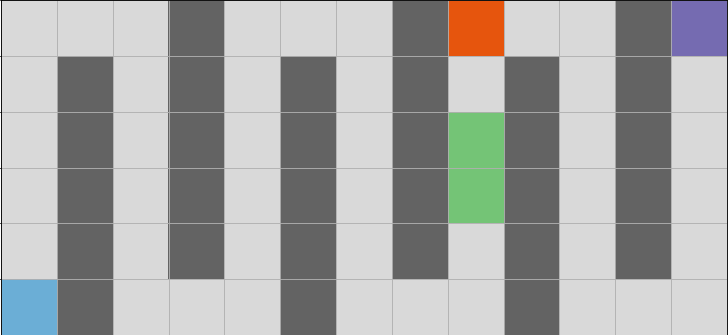
\includegraphics[width=\textwidth]{./figs/world-simple-maze}
	\end{center}
\end{frame}

\begin{frame}
	\frametitle{Roboworld}
	\begin{center}
		Roboworld Demo: \href{https://datahub.cs.hm.edu/}{https://datahub.cs.hm.edu/}
	\end{center}
\end{frame}

\subsection{Minimale technische Hürden}

\begin{frame}
	\frametitle{JupyterHub}
	Eigener JupyterHub auf unserem Kubernetes-Cluster:
	\begin{figure}
		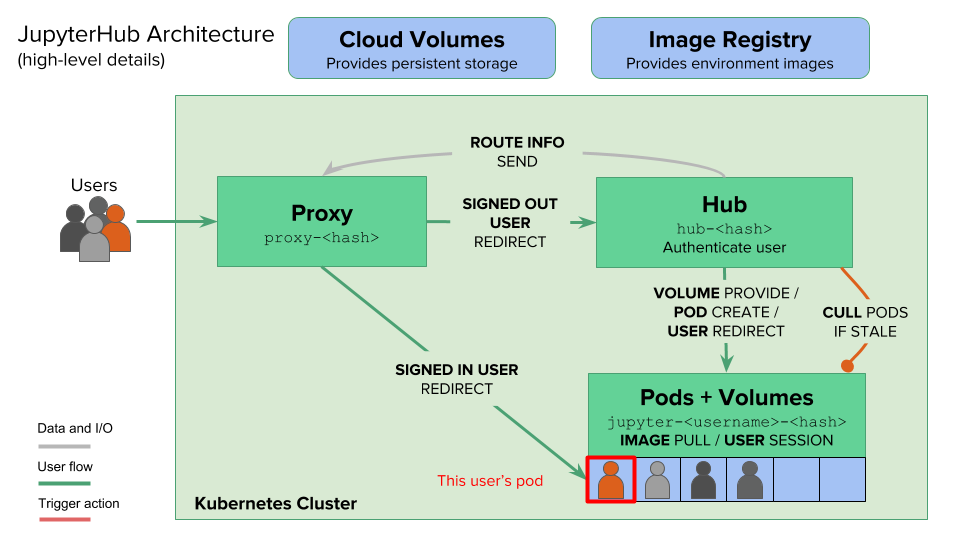
\includegraphics[width=0.75\textwidth]{./figs/infrastructure}
		\caption{Quelle: \href{https://zero-to-jupyterhub.readthedocs.io/en/latest/administrator/architecture.html}{The JupyterHub Architecture}}
	\end{figure}
\end{frame}

\begin{frame}
	\frametitle{JupyterHub}
		\begin{block}{Minimale technische Hürden}
	Vorteile:
	\begin{enumerate}[label = $\bullet$]
		\item einheitliche vorkonfigurierte Entwicklungsumgebung
		\item Aufgabenverteilung durch git (im Hintergrund)
		\item starke Gemeinschaft
		\item Rechenleistung auf Serverseite
	\end{enumerate}
Nachteile:
\begin{enumerate}[label = $\bullet$]
	\item keine individuelle Entwicklungsumgebung
	\item fehlende Interaktion mit git-Befehlen
	\item keine Funktionalität für Abgaben (Praktikum, Prüfung)
	\item Rechenleistung auf Serverseite (ab ca. 100 Benutzer:innen wird Kubernetes benötigt)
\end{enumerate}
\end{block}
\end{frame}

\subsection{Kontinuierliches Feedback}

\begin{frame}
	\frametitle{Otter-Grader}
	\begin{center}
		Otter-Grader Demo
	\end{center}
\end{frame}

\begin{frame}
	\frametitle{Otter-Grader}
	\begin{block}{Kontinuierliches Feedback}
			Vorteile:
		\begin{enumerate}[label = $\bullet$]
			\item realisiert \textbf{kontinuierliches Feedback} für Studis
			\item einfach zu bedienen (für Lehrende als auch für Studis)
			\item Code, Aufgabenstellung und Tests in einem Dokument
		\end{enumerate}
		Nachteile:
		\begin{enumerate}[label = $\bullet$]
			\item funktioniert ausschließlich mit Notebooks
			\item Auto-Grading ist nicht voll automatisiert
			\item (sichtbare) Tests werden mitgeliefert
		\end{enumerate}
	\end{block}
\end{frame}

\begin{frame}
	\frametitle{Jupyter-Book}
	\begin{center}
		\href{https://bzoennchen.github.io/ct-book/intro.html}{CT-Jupyter-Book Demo}
	\end{center}
\end{frame}

\begin{frame}
	\frametitle{Retrospektive}
	\begin{enumerate}[label = $\bullet$]
		\item Besserer Dialog zwischen Lehrende und Lernende notwendig (insbesondere während der Pandemie)
		\item Noch mehr ``Doing'' der Studis
		\item Zu Beginn kleinteiligere Problemstellungen		 
		\item Programmiersprachenspezifika unvermeidbar?
		\item Tempo musste gedrosselt werden
		\item Python + Jupyter-Ökosystem eignen sich für CT		
	\end{enumerate}
\end{frame}

\appendix

\begin{frame}[plain]
	\frametitle{Quellen}
	\begin{enumerate}[label = ]
		\item Jupyter-Book: \href{https://bzoennchen.github.io/ct-book/intro.html}{https://bzoennchen.github.io/ct-book/intro.html}
		\item Roboworld Doku: \href{https://robo-world-doc.readthedocs.io/en/latest/index.html}{https://robo-world-doc.readthedocs.io/en/latest/index.html}
		\item Vortragsunterlagen: \href{https://github.com/BZoennchen/fdak-sep}{https://github.com/BZoennchen/fdak-sep}
		\item Otter-Grader: \href{https://otter-grader.readthedocs.io/en/latest/}{https://otter-grader.readthedocs.io/en/latest/} 	
		\item JupyterHub: \href{https://jupyter.org/hub}{https://jupyter.org/hub}
		\item Jupyter-Notebooks: \href{https://jupyter.org/}{https://jupyter.org/}
	\end{enumerate}
\end{frame}

%\begin{frame}
%	\frametitle{Lessons}
%\end{frame}

\end{document}
